% \documentclass{ijsra}
\def\IJSRAidentifier{\currfilebase} %<---- don’t change this!
\def\submission{}%YYYY-MM-DD
\def\acceptance{}%YYYY-MM-DD
%-------Title | Email | Keywords | Abstract-------------
\def\shorttitle{Robben Island}
\def\maintitle{Robben Island: Representation and Interpretation of the materiality of apartheid and imprisonment}
\def\cmail{ephrainmmwaita@gmail.com}
\def\keywords{Apartheid, Imprisonment, material culture}
%\def\keywordname{}%<--- redefine the name “Keywords“ in needed language
\def\abstract{This paper examines the symbolic interpretations and material representations of the apartheid political imprisonment period on Robben Island (South Africa). It is a critical archaeology of conflict, examining what survives, why is that material record important, and what mechanisms exists for retaining its significance in a form that can benefit present and future generations
 \parencites[1]{Howard1994}[Carman 1997 in][]{Beck_2004}.
 % (Howard 1994:1; Carman 1997 in Beck et al. 2003).
Robben Island Museum presents a narration of inhumane political imprisonment, based on the oral histories and memory of former political prisoners, with much emphasis on the ‘triumph’ of political prisoners in enduring the inhumane prison conditions. Little is being done to engage with the inhumane practices of Robben Island apartheid political imprisonment through the use of material culture objects. Although the values we place on material culture objects are diverse, material culture objects usually provide an experience that is substantially different from oral histories, as oral histories and memory tend to change with space and time. Therefore, this paper intends to connect these oral histories and memories to material culture objects so that they too are part of the apartheid political imprisonment story.}
%--------Author’s names------------
\def\authorone{Ephraim Mwaita}
%-------Biographical information-------------
\def\bioone{Ephrain Mwaita studied for a Post Graduate Diploma in Museums and Heritage at the University of the Western Cape, and is currently enrolled for a Master of Arts at Swansea University. He is also a tour guide for the Robben Island Museum, and has designed and curated an exhibition for Robben Island titled "Robben Island: The horror of our past". He has attended research workshops for the Southern Africa Students Council (SASC) and the Association of Southern Africa Professional Archaeologist (ASAPA), discussing his research on Robben Island.}
%------University/Institution--------------
\def\affilone{Swansea University}

\begin{filecontents}{\IJSRAidentifier.bib}
	@article{Howard1994,
author= {Howard, P.},
journal= {International Journal of Heritage Studies},
volume= {1},
number= {1},
year={1994},
title= {The Heritage Discipline},
pages= {1-3},
}


@article{Alberti_2000,
	author = {Alberti, S.},
	journal = {Isis},
	number = {4},
	pages = {559-571},
	title = {Objects and the Museum},
	volume = {96},
	year = {2000},
}

@book{Alexander_1994,
	address = {Cape Town},
	author = {Alexander, N.},
	publisher = {UCT Press},
	title = {Robben Island prison dossier 1964-1974},
	year = {1994},
}

@book{Beck_2004,
	address = {London},
	editor = {Beck, C. M. Johnson and W. J. Schofield W. J. Schofield},
	publisher = {Routledge},
	series = {One World Archaeology},
	title = {MatÈriel Culture: The Archaeology of Twentieth-Century Conflict},
	volume = {44},
	year = {2004},
}

@book{Foucault_1995,
	address = {New York},
	author = {Foucault, M.},
	publisher = {Vintage Books, Random House},
	title = {Discipline and Punish: the birth of the prison},
	date = {1995},
origdate = {1977}
}

@book{Harrison_2010,
	address = {Manchester},
	editor = {Harrison, R},
	publisher = {Manchester University Press and Open University Press},
	title = {Understanding the Politics of Heritage},
	year = {2010},
}

@article{Haslam_2014,
	author = {Haslam, N. and Loughnan, S.},
	journal = {The Annual Review of Psychology},
	pages = {399-423},
	title = {Dehumanization and Infrahumanization},
	volume = {65},
	year = {2014},
}

@incollection{Hoskins_2006,
	address = {Routledge,},
	author = {Hoskins, J.},
	booktitle = {Handbook of Material Culture},
	editor = {Tilley, C. et al},
	pages = {74-84},
	publisher = {London},
	title = {Agency, Biography and Objects},
	year = {2006},
}

@book{Hutton_1997,
	address = {Johannesburg and Bellvile},
	author = {Hutton, B.},
	publisher = {SACHED and Mayibuye Books},
	title = {Robben Island: Symbol of Resistance},
	year = {1997},
}

@book{Robben_2012,
	address = {Cape Town},
	publisher = {Robben Island World Heritage Site},
	title = {Integrated Conservation Management Plan: Abridged Version},
	date = {2007/2012},
}

@book{Robben_2013,
	address = {Cape Town},
	publisher = {Robben Island World Heritage Site},
	title = {Integrated Conservation Management Plan: Abridged Version},
	date = {2013/2018},

}

@book{Red_2009,
	address = {Pretoria},
	author = {International Committee of the Red Cross},
	publisher = {Red Cross Regional Delegation of South Africa},
	title = {Commemorating 150 years since the battle of Solferino: 24 June 1859-24 June 2009},
	year = {2009},
}

@techreport{ICOM_2007,
	author = {ICOM},
	institution = {International Council of Museums},
	note = {Accessed on 09 December 2016},
	title = {Museum Definition},
	year = {2007},
	url = {http://icom.museum/the-vision/museum-definition/},
}

@article{Martin_2009,
	author = {Martin, L. L and Mitchelson, M. L.},
	journal = {Geography Compasses},
	number = {1},
	pages = {459-477},
	title = {Geographies of Detention and Imprisonment: Interrogating Spatial Practices of Confinement, Discipline, Law and State Power},
	volume = {3},
	year = {2009},
}

@book{Naidoo_1982,
	address = {Penguin books},
	author = {Naidoo, I.},
	publisher = {Cape Town},
	title = {Island in Chains},
	year = {1982},
}

@mastersthesis{Nesje_2005,
	author = {Nesje, P.},
	school = {University of Cape Town},
	title = {Representing the Past in the Present with the Future in Mind: A Close Reading of the Cell Stories Exhibition at the Robben Island Museum},
	year = {2005},
}

@article{Rafael_2005,
	author = {Rafael, T.},
	journal = {Journal of the American Institute for Conservation},
	number = {8},
	pages = {245-257},
	title = {Preventive conservation and the exhibition process: development of exhibit guidelines and standards for conservation},
	volume = {33},
	year = {2005},
}

@book{Rioufol_2000,
	address = {Cape Town},
	author = {Rioufol, V.},
	publisher = {University of the Western Cape Press},
	title = {Behind Telling: Post-Apartheid Representations of Robben Island's Past},
	year = {2000},
}

@mastersthesis{Rioufol_1999,
	author = {Rioufol, V.},
	school = {University of Cape Town},
	title = {The Making of the New Past for a "New" South Africa: the commemoration of Robben Island},
	year = {1999},
}

@book{Robben_2003,
	address = {Cape Town},
	author = {Robben Island Museum Ex-Political Prisoners Reference Groups},
	publisher = {Robben Island Museum},
	title = {Project Blue Stone Quarry},
	volume = {2},
	year = {2003},
}

@article{Solani_2000,
	author = {Solani, N.},
	journal = {Kronos: The Journal of Cape History},
	number = {5},
	pages = {42-55},
	title = {The Saint of the Struggle: Deconstructing the Mandela Myth},
	volume = {26},
	year = {2000},
}

@unpublished{SAMA_2007,
	author = {SAMA (sama)},
	title = {Policy Adopted during the 21st General Conference of the South African Museums Association in Vienna},
	year = {2007},
}

@book{Walker_2013,
	author = {Walker, Meredith},
	edition = {7th},
	publisher = {ICOMOS},
	title = {The Burra Charter: The Australia Icomos Charter for the Conservation of Places of Cultural Significance},
	year = {2013 (1979)},
}

@unpublished{Wintein_2015,
	author = {Wintein, C.},
	title = {Robben Island Site Collection Report 1998-2014},
	year = {2015},
}
\end{filecontents}
\IJSRAopening%<---- don’t change this!
%-------
\lettrine{R}{obben} Island is in Table Bay, 6.9 km west of the coast of Bloubergstrand, Cape Town, South Africa, with coordinates of 33.8076$^{\circ}$ S, 18.3712$^{\circ}$ E as seen in Figures \ref{fig:Mwaita_Figure_01}, \ref{fig:Mwaita_Figure_02}, and \ref{fig:Mwaita_Figure_03} below. The name ‘Robben’ is a Dutch word ‘Robbe’ meaning ‘Seal’. The island was named after the seals which are found around the island.

%FIGURE 1:
\begin{figure}[!htb]
	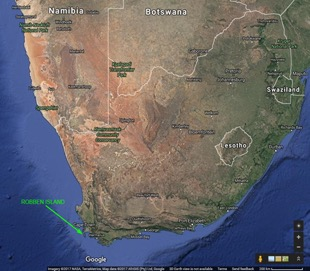
\includegraphics[width=\linewidth]{Mwaita_Figure_01}
	\caption{Location of Robben Island in Southern Africa
  {\normalfont\scriptsize \\ \copyright\ by
                   Google Satellite Maps 2017, image created by the author). Available from: \url{https://www.google.co.za/maps/search/robben+island+museum+in+africa/@-27.2742339,18.2402094,1887137m/data=!3m1!1e3?hl=en}. (Accessed on 11 February 2017).
                    }}
	\label{fig:Mwaita_Figure_01}
\end{figure}

%FIG2
\begin{figure}[!htb]
	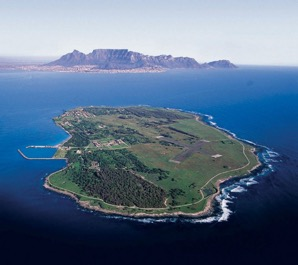
\includegraphics[width=\linewidth]{Mwaita_Figure_02}
	\caption{Aerial view of Robben Island with Table Mountain in the background
  {\normalfont\scriptsize \\ \copyright\ by
      South African History online \url{http://www.sahistory.org.za/sites/default/files/u7/robben-island-pic.jpg}) Accessed on 09 February 2017).
                    }}
	\label{fig:Mwaita_Figure_02}
\end{figure}

%FIG3
\begin{figure}[!htb]
	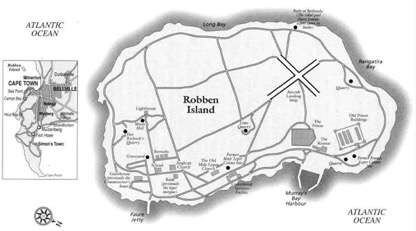
\includegraphics[width=\linewidth]{Mwaita_Figure_03}
	\caption{Robben Island map
  {\normalfont\scriptsize \\ \copyright\ by
                    Source:  Cape Town heritage website: \url{http://www.cape-town-heritage.co.za/img/robben-island-map.jpg}. (Accessed on 09 February 2017)
                    }}
	\label{fig:Mwaita_Figure_03}
\end{figure}


Robben Island was declared a National Museum in 1996 and a World Heritage Site in 1999. It is a living museum with the vision of making sure that the history of Robben Island is remembered and promoted as a unique symbol of the “triumph of the human spirit over hardship and injustice” \parencite{Robben_2012} (Fig. \ref{fig:Mwaita_Figure_04}). Although Robben Island Museum’s status as a World Heritage Site derives from a far longer history, as a place of banishment, confinement, armament, and settlement, it is most popularly known through apartheid history, as a place of imprisonment.

%FIG 4 AB
\begin{figure}[!htb]
	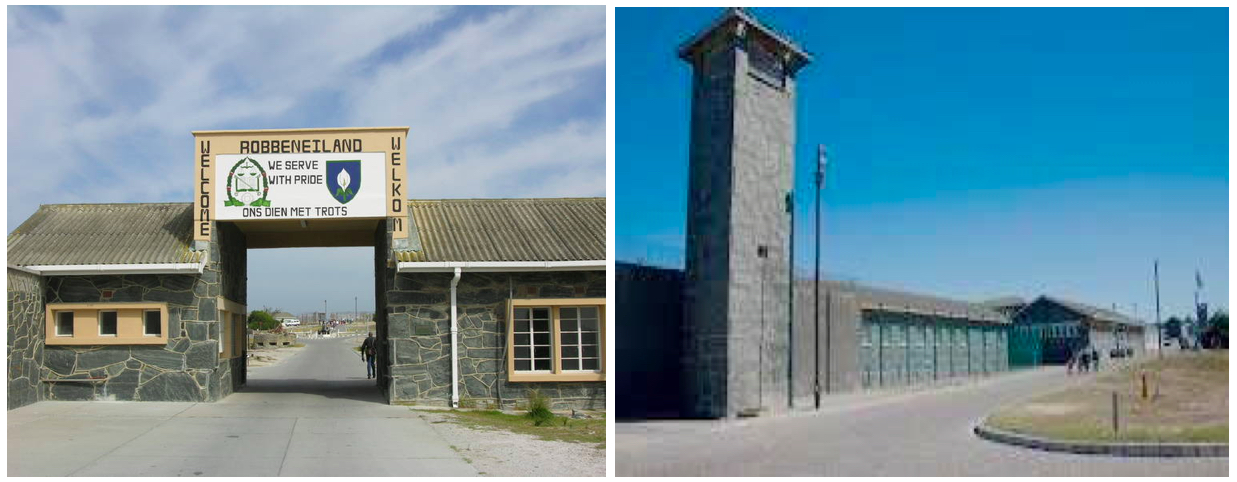
\includegraphics[width=\linewidth]{Mwaita_Figure_04}
	\caption{Robben Island Museum: (left) entrance to the prison from the harbour, and (right) a view of the maximum prison
  {\normalfont\scriptsize \\ \copyright\ by
Images taken by the author with permission of the Museum
                    }}
  	\label{fig:Mwaita_Figure_04}
\end{figure}

Many scholars \parencites{Hutton_1997}{Nesje_2005}{Rioufol_2000}{Solani_2000} have argued over the interpretive narratives of Robben Island. In support of the apartheid narrative \textcite{Rioufol_2000} and \textcite{Solani_2000} state that, in the creation of a unified national identity, a reconciliatory image, one of ‘the triumph of human spirit’, was chosen at the expense of a broader apartheid narratives as witnessed on the museum’s statement of significance by Ahmed Kathrada:

\blockcquote[17]{Robben_2012}{While we will not forget the brutality of apartheid, we will not want Robben Island to be a monument to our hardship and suffering. We would want it to be a triumph of the human spirit against the forces of evil. A triumph of wisdom and largeness of spirit against small minds and pettiness; a triumph of courage and determination over human frailty and weakness, a triumph of the new South Africa over the old… }

However, this triumphant narrative, and its focus on memory-makers, influential political inmates such as Nelson Mandela and Ahmed Kathrada, neglects the broader apartheid prison experience of inhumanity.

In this paper, I present the inhumanity of apartheid political imprisonment through the use of material culture objects. In presenting these objects I hope to address the imbalances of the Robben Island museum narrative. Furthermore, I discuss the role of museums, as national institutions of knowledge, nation building, and as an instrument of power in confronting the ills of the past.

\IJSRAsection{Current Museum Apartheid Narrative}

\textcite{Solani_2000} explains that the Museum perpetuates the Mandela myth, despite Robert Sobukwe’s, the founding president of the Pan African Congress (PAC), house being located in the prison yard, rather much of the attention is paid to Nelson Mandela: his cell and labour in the lime quarry and the courtyard. From my experience as a tour guide in 2015, I noticed visitors were not taken to the Blue Stone Quarry, which is where most of the brutality took place and where the majority of prisoners worked during the 1960's. This focus, as \textcite{Rioufol_1999} points out, on influential memory-makers neglects the broader apartheid political imprisonment narrative. Accordingly, this focus neglects a broader selection of spaces and material culture available to the museum and the agency of materials to narrate the imprisonment experience.

Within this ‘triumphant’ narrative the museum prioritizes oral accounts over movable material culture. Although ex-political prisoners are tour guides on the Island who share their experiences during their time of imprisonment, this alone is not enough in fostering the story of the individual, everyday-lived experiences of political prisoners on the Island. However, there has been some effort to include material culture objects in the Museum narrative, especially in the house of Robert Sobukwe (Pan African Congress Leader) and in most of the prison cells. Nonetheless, there remain many spaces that are not filled by objects that could enhance the museum narrative of the everyday life of imprisonment, for instance, in the hospital, kitchen, or church. This gap in the narrative can be addressed by the physical evidence of movable material culture objects that can mediate between the past and the present.

Movable material culture objects have not played a prominent role in the story of apartheid political imprisonment at Robben Island. The second \textcite{Robben_2013}, argues that the first ICMP Interpretation Plan was not properly implemented, possibly because it was considered too complex and, therefore, difficult to implement. This has produced an ineffectual communication of the histories of Robben Island by not developing the relationship between tangible and intangible heritage. The relationship between tangible and intangible heritage is the attachment of memories on objects in order to let objects speak for themselves, whereby the objects are tangible representations of intangible heritage \parencite{Hoskins_2006}.

Robben Island Museum is the custodian of historical objects that were left on the Island by the prison authorities, such as picks, hammers, spades, and ropes \parencite{Wintein_2015}. These objects are locked in storerooms; consequently, few of these objects, arguably central to narrating the inhumanity of Robben Island political imprisonment, have been exhibited to the public. Therefore, I chose to document and present these objects.

\IJSRAsection{Method}

In carrying out the research, I consulted published and unpublished written records, as well as audio and video interviews of former apartheid political prisoners at Robben Island-Mayibuye Archives. I also attended numerous guided tours with different tour guides to have an understanding of the background of the museum and how it is presented to the public. Museum Collections and Conservation Unit Manager, Ms Caroline Wintein, gave me the Permission under a request from the University of the Western Cape and Robben Island Education Department to tour Museum storage rooms and to take photographs of objects for research purposes. I could have expanded my research to produce a broader narrative of apartheid political imprisonment on the Island by including other material culture objects at neglected sites such as the hospital, workshop, sports field, kitchen, and agriculture, but I had limited time to complete my research in the fulfilment of my Post Graduate Diploma in Museums and Heritage Studies.

\IJSRAsection{ROBBEN ISLAND APARTHEID INTERPRETATIONS}

\IJSRAseparator

\IJSRAsection{Apartheid South Africa}

South Africa witnessed segregation and discrimination from 1948 to 1994, the then government passed discriminatory laws to control every aspect of black people’s lives, laws about where people could live, work, trade, and learn. Severe measures were taken against those who resisted, and those who fought against these laws were arrested and incarcerated on Robben Island from 1960 until 1991.

Before 1970 most prisoners were sentenced to hard labour working in either the stone or lime quarries, collecting seaweed in the ice-cold sea, and breaking rocks into smaller pieces. Failure to fulfil the quota was punished by having to complete additional labour, such as building roads, clearing fields, and chopping wood. In the process of hard labour, prisoners were also assaulted, beaten with ‘baton sticks’ \parencite[54]{Hutton_1997}.

Racial discrimination continued within the prison. Black prisoners were treated differently from Coloured or Asian prisoners, and received less food and clothes. However, organization, discipline, and courage kept political prisoners alive, they fought the brutality and harsh prison conditions through the establishment of committees, such as disciplinary, educational, political, and recreational \parencite[55]{Hutton_1997}.

Robben Island, during the period of 1962 to late 1970's, became an International concern for human rights violations; it has been extensively documented, more particularly by certain International organizations. Evidence on the conditions and treatment of political prisoners at Robben Island during this period was given to the United Nations Commission for Human Rights and the special Political Committee on apartheid \parencites{Alexander_1994}{Red_2009}.
In South Africa Mayibuye archives is one of the Institutions with rich literature and oral histories describing the inhumane nature of apartheid political imprisonment. \textcite[21]{Alexander_1994}, described Robben Island as a “microcosm of apartheid violence and injustice”. This shows how inhumane apartheid imprisonment was and a turning point into a new post-apartheid South Africa.

\IJSRAsection{Post-Apartheid South Africa}

Debates took place as a way of constructing the interpretation of Robben Island to the public and the need for a conciliatory narrative was raised and adopted. The Heritage Site became to be regarded as ‘the birth of a new and democratic South Africa’ and the liberation movement narrative was adopted to interpret the site as the triumph of the human spirit over brutality, the triumph of wisdom, courage and determination over oppression \parencite[62--63]{Robben_2012}.

This narrative was drawn at the same time South Africa was embarking on the reconciliation strategy, during the political transition from apartheid to a ‘new’ free and democratic society in which Nelson Mandela became the influential figure and the symbol for the transition. Reconciliation, peace and democracy were preached across the country under the influence of key political figures, former political prisoners. \textcite[43--48]{Nesje_2005}, argued that the interpretation of Robben Island was highly politicized. I concur with her in the sense that the key and most influential figure in the making of Robben Island as a museum, Ahmed Kathrada, was the personal advisor to Nelson Mandela, the brains behind reconciliation in the new democratic South Africa.

In support of this narrative the ‘Esiqithini’ exhibition in 1993 was redisplayed in 1996 and changed its name to Robben Island Gateway project focusing on the prisoner’s resistance and resourcefulness. The exhibition focused on political prisoners, those before the apartheid era such as the Khoisan, Xhosa, Koranna, Zulu chiefs, Muslim leaders from India and those during the apartheid era. The pre-apartheid era section of the exhibition focuses on the political prisoners struggle for freedom, poor living standards, ill-treatment, escape attempts and sea drowning, During apartheid era imprisonment, the exhibit focused on how the political prisoners arranged themselves in fighting for the improvement of conditions in the prison and how they were receiving messages of sympathy and admiration from international and national anti-apartheid groups \parencite{Nesje_2005}.

The ‘Cell Stories’ exhibition, which was displayed at Nelson Mandela gateway to Robben Island, narrated how prisoners endured and adapted to the brutality and harsh conditions by turning the prison into a ‘University’, thus focusing on individual achievements. The exhibition was made up mainly with objects belonging to individuals such as books made of cement bags, waist belt made of sea weed, shoes made of hare skin, sports and academic certificates attained in the prison, the long march to freedom script by Nelson Mandela, sisal mates and woodworks, as well as other objects donated to the museum by former political prisoners \parencite{Rioufol_1999}.

In September 2015, I had the opportunity to view the “Journeys of Sorrow and Hope” permanent exhibition, which is displayed at Robben Island Museum Jetty 1. The exhibition explains the place as the embarkation point to and from the Island by political prisoners, visitors, and warders. Inside the historic building, letters of family members, church groups, social services organizations, and legal personnel’s seeking permission to visit political prisoners are displayed on the wall as are letters confirming the permission. Photographs of different people who went to Robben Island during apartheid political imprisonment including prisoners, warders, and visitors, are also on display. On the display again is the reference group, these are women mostly wives of political prisoners who managed to visit their husbands on the Island sharing their experiences, how they manage to get travel funds, struggling and failing to have accommodation when they arrive in Cape Town, the harshness of their ferry journey’s to and from the Island, and the sad journey back to their homes.

These exhibitions illustrate the ‘triumphalism’ narrative. From the above exhibitions it can be noted that there is ineffective confrontation of the past horrors considering the selection of objects for the exhibitions and their themes. Most of the prison materials such as picks, wheel barrows, hand axes, shovels, the ‘mary’, handcuffs, baton sticks, cane, crockery, bedding and prison clothes are not utilized to tell their stories at Robben Island. In reality did every political prisoner achieve something as a result of imprisonment? I argue that the ‘triumphant’ narrative does not commiserate those who died or suffered in their health as a result of the inhumane treatment. The political stanza of reconciliation affected the complete representation of Robben Island as a museum to the public in downplaying other memories of the inhumane reality of apartheid political imprisonment as well its legacy in present and future generations.

\IJSRAsection{The agency of objects}

\blockcquote[24]{Hoskins_2006}{The lines between persons and things are culturally viable [and] in certain contexts, persons can seem to take on the attributes of things and things can seem to act almost as persons}

Contemporary discussions about the politics of memory are concerned with doing justice to forgotten voices and victims. With such it is important for the Museum to include tangible objects that were left on the Island that serve as the evidence of the intangible events of the brutality that took place on the Island during apartheid political imprisonment.

\textcite{Hoskins_2006} further argues that the analysis of material culture objects can be used to interpret human activities in relation to their environment since these materials are culturally made by humans to serve humans. Objects are agents specifically made for a purpose to foster the relationship between humans and the natural environment.
\textcite[32--35]{Alberti_2000} also argues that objects act as primary sources of the unseen events of the past. Therefore, objects can be used as the evidence in the study of past events.
\textcite{Harrison_2010} formulates a theory about the creation of objects that could in fact be a theory about the creation of all forms of material culture, he asserts that things are made as a form of instrumental action; objects are produced in order to influence the thoughts and actions of others.

According to the International Council of Museums (ICOM) and South African Museum Association (SAMA) a museum object tells a story through its physical structure and its associations, it is this which determines the value of an object to a museum, and core functions of museums includes research, on collections in order to generate knowledge and on the repacking of existing information and data in ways that make people think, appreciate, and communicate. This process includes the creation of relationships between people and museum objects either through exhibitions, public events, educational programmes, pamphlets, social media, publications, newspaper or magazine articles, as a way to make people participate and respond.

The Robben Island museum is doing an injustice to its collections, which can tell the brutality of apartheid political imprisonment because these important objects are not being used in the interpretation of the museum. I now will provide a counter narrative to the museum’s interpretation by outlining material culture objects that depicts the horrors and inhumane nature of apartheid political imprisonment on Robben Island. In so doing, I make use of memories and oral history as a way to attach meanings on objects and establish their importance and value museum narrative.

\IJSRAsection{Material culture objects of political imprisonment}

%Fig 5

\begin{figure}[!htb]
	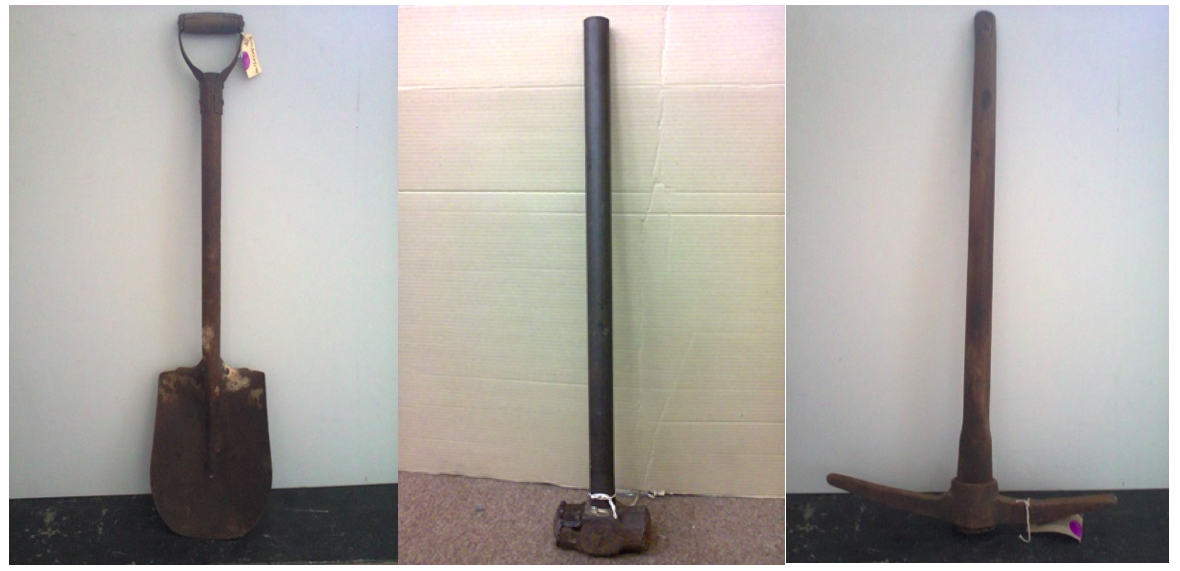
\includegraphics[width=\linewidth]{Mwaita_Figure_05}
	\caption{Hard Labour objects: (left to right) shovel, hammer and pick axe
  {\normalfont\scriptsize \\ Source: Robben Island Museum, Images taken by the author with permission of the museum
                    }}
	\label{fig:Mwaita_Figure_05}
\end{figure}


Generally pick axes, shovels, hammers, and wheel barrows are used to make tasks that are ordinarily difficult significantly easier (see \cref{fig:Mwaita_Figure_05}).
Pick axes used to break up soils that a shovel cannot, hardened clay or rocky soils, hard surfaces such as cement, tile and ice can be broken up using the sharp end of the axe or a hammer, whilst a wheel barrow is used in nearly every country in the world for construction, roadwork, masonry and landscaping. Wheel barrows are essential, helping take the load off your back and can be used to transport supplies, tools, compost or debris to and from one place to the other. On Robben Island, however, these objects serve as evidence to the brutality of political imprisonment on the island considering their associations. Hutton wrote:

\blockcquote[Michael Dingake in][57]{Hutton_1997}{It was hard work at the stone quarry, compressor drills vibrated the whole day, shaking their operators like reeds in the wind. Some prisoners wielded huge hammers and pounded metal pins with all their might to split huge rocks embedded below sea level. The bulk of prisoners sat in arranged groups to break the rock pieces into smaller pieces, failure to fulfil the quota were punishable. The rest of the work span carted the crushed stones around in wheelbarrows. Blisters and callused hands were the hallmarks of quarry span prisoners.}

Hutton also wrote about the experience on the lime quarry of Helao Shityuwete of SWAPO who was sentenced to 16 years. Hutton (1997:57) describes Helao’s experience on the lime quarry:

\blockcquote[57]{Hutton_1997}{ …we were sent to work in the two lime quarries, chipping away at the rock-face with only picks, shovels and spades. It was very hard work and a drizzling glare came off the white rocks when the sun shone as we had no sunglasses, the eyesight of many of us was damaged.}

\textcite[76]{Naidoo_1982} also points out that beside the quarries, these material objects have also been used by political prisoners in other various works such as making and repairing roads, dragging seaweed from the beaches and from the sea, clearing fields, and chopping wood.

According to \textcite[131]{Alexander_1994}, from 1962 to 1964 brutal assaults of political prisoners were a weekly, often a daily occurrence. Baton sticks represent such assaults during apartheid political imprisonment. \textcite[131]{Alexander_1994} further reiterates that, in the early years of imprisonment most of the warders were indoctrinated such that they actually believed that black people were animals, not humans, and those warders were abusive and quick to react in beatings. A number of prisoners, including Andrew Masondo (a former lecturer in Mathematics at Fort Hare University College) and Dennis Brutus were severely wounded, with Brutus carrying the scars of that day on his body \textcite[132]{Alexander_1994}.According to \textcite[52]{Hutton_1997} Michael Dingake, a former political prisoner shared his experience on the use of the baton stick during apartheid imprisonment:

\blockcquote[52]{Hutton_1997}{Armed with batons they raided our single cells in batches of three and four. ‘Teen die murr!’ (Against the wall!) ‘Trek uit.’ (Strip). A number of prisoners in the segregation section were assaulted…Andimba Toivoja Toivo, the SWAPO leader was one of those who was severely beaten. After the assault, like the other victims of that \nth{28} day of May 1971 he was forced to clean his blood-spatted cell.}

\textcite[28]{Alexander_1994} also narrated the same incident \enquote{Japhtha Masemola was beaten unconscious, while Abel Chiloane was so severely injured that for days he urinated blood.}

The ‘mary’ and ‘bamboo cane’ (see \cref{fig:Mwaita_Figure_06}) depicts severe and cruel maltreatment during imprisonment. According to Indres \textcite[22]{Naidoo_1982}, the ‘mary’ is a wooden frame like a ladder with a foot stand and hand holders on its sides as seen in figure 4.1. This instrument has its origins in the medieval period in Europe and was used for torture. Indres Naidoo, imprisoned on Robben Island in 1963 and serving ten years, is one of the victims of the ‘mary’. The punishment was done whilst the prisoner is naked. Indres Naido reiterated that after he was severely caned he had difficulty sitting and could only sleep, lying on his stomach, for about three weeks \parencite{Naidoo_1982}.

%Fig 6 AB
\begin{figure}[!htb]
	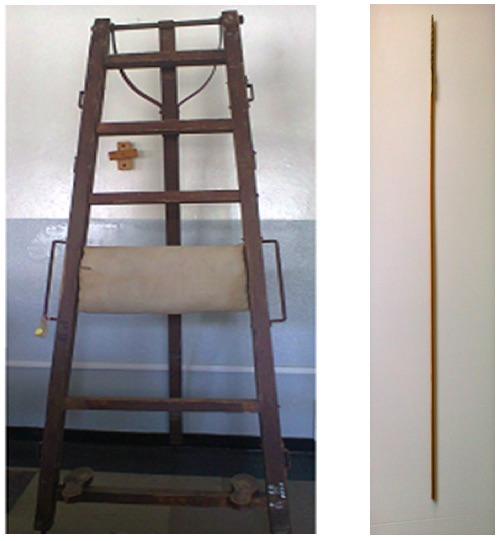
\includegraphics[width=\linewidth]{Mwaita_Figure_06}
	\caption{Torture Objects: the "mary" (left) and the bamboo cane (right).
  {\normalfont\scriptsize \\   Source: Robben Island Museum, Images taken by the author with permission of the museum.
                    }}
	\label{fig:Mwaita_Figure_06}
\end{figure}

Prison clothes depict the racial classification of political prisoners inside the prison. \textcite{Alexander_1994}, postulates that black prisoners were given short pants with no underwear, short sleeve shirts, and sandals even in winter, with a large number of black inmates forced to go barefoot for most of the year. Coloureds and Indians were given long pants, shoes and stockings. If a doctor authorized it, certain African prisoners were given ‘Coloured’ clothing for reasons of health. \textcite{Alexander_1994} also reiterated that there was no adequate clothing, each prisoner was given one pair of clothes and shoes or sandals and in most cases when something was alleged to be out of stock or, for instance, when a broken shoe or sandal had to be repaired, in such cases a prisoner was going to be under clothed, and sometimes prisoners were forced to go and work in the rain without the protection of waterproof coverings. This shows the psychological effects of humiliation especially to black political prisoners. Mac Maharaj \parencite[in][62]{Hutton_1997} described prison clothes, “It used to be made out of khaki and sailcloth, with one thin jersey given to you on 25 April and taken away on 25 September irrespective of whether it was going to be hot or cold in the intervening period...”.

Sisal mats as seen in Figure \ref{fig:Mwaita_Figure_07}, blankets, mattresses and beds depict the harshness of bedding during apartheid political imprisonment period. Alexander (1994) postulates that “bedding was inadequate, three blankets were issued to all prisoners in the early years usually in the worst possible condition, old, thin, dirty, and smelly things that ought to have been condemned years before”. At the same time non-political prisoners enjoyed a proper set of blankets, while black inmates were not given beds unless they became ill, they slept on sisal and felt mats.  In addition, Mac Maharaj, (in Hutton 1997: 61) also states that no bedding in the form of bed sheets, pillows, bedspreads or pyjamas were provided for black political prisoners.

%Fig 7
\begin{figure}[!htb]
	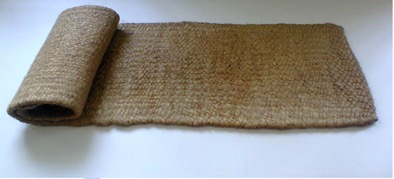
\includegraphics[width=\linewidth]{Mwaita_Figure_07}
	\caption{Cruelty treatment: Sisal mate
  {\normalfont\scriptsize \\ Source: Robben Island Museum, Image taken by the author with permission of the museum
                    }}
	\label{fig:Mwaita_Figure_07}
\end{figure}

Censored letters also depict another form of psychological torture during political imprisonment. Most of the political prisoners received their letters with information cut off and in some cases a prisoner can just see the greetings and salutations of the letter with all the content chopped off by prison authorities. In my view, this is denying one’s liberty, as Foucault attributed ‘deprivation of liberty’ as one of the inhumane prison conditions: “in which liberty is a good that belongs to all in the same way and to which each individual is attached” \parencite[232]{Foucault_1995}. As a result, this affects psychologically, as one can have more questions than answers regarding the actual content of the letter, and can create mental instability to the receiver of the letter.

Although plates, cutlery and cups were the same, the food was not the same, again there was segregation in terms of race as illustrated in Table \ref{fig:Mwaita_Table_01}. Racism kept the prisoners divided, to break solidarity and unity among political prisoners. Racial segregation can be viewed as a prison inside the prison to black prisoners and as a diplomatic move to separate or to make political prisoners hate each other as a way of avoiding future co-operation and unity among political prisoners in the prison. According to \parencite[47]{Hutton_1997}, when Robben Island became the maximum prison of political imprisonment, all the Warders were white with black prisoners either Coloured or Asian, and \textcite[131]{Alexander_1994} reiterates that, “in the early years of imprisonment most of the warders were indoctrinated such that they actually believed that black people were hardened prisoners, and those warders were abusive and quick to punish.”

%Table
\begin{figure}[!htb]
	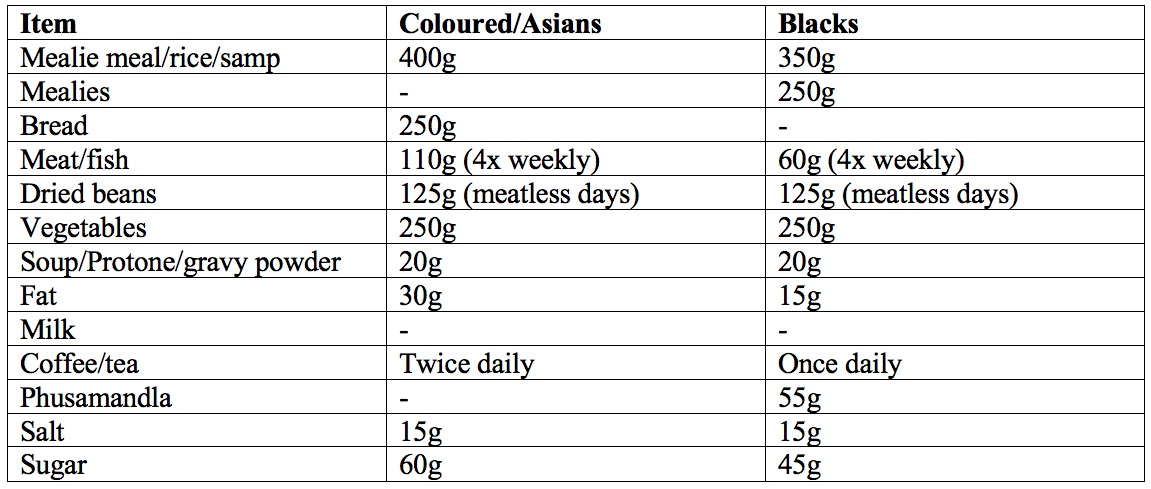
\includegraphics[width=\linewidth]{Mwaita_Table_01}
	\caption{Adapted from the description of political prisoner’s meals by Michael Dingake in Hutton (1997:54).
	}
	\label{fig:Mwaita_Table_01}
\end{figure}

Sanitary buckets in Figure \ref{fig:Mwaita_Figure_08} depict the harshness of the prison. \textcite[67--68]{Naidoo_1982} writes that in the 1960's single cells of section B had no toilets so political prisoners kept in that section, mostly leaders, were using the bucket system to relieve themselves but were forced to use the same bucket for bathing. This shows a great deal of dehumanization, reducing human beings to a level lower than animals. Indres Naidoo even stated that sometimes they were even called ‘pigs’ by prison warders \parencite{Naidoo_1982}.
\textcite{Haslam_2014} highlight that people tend to perceive out-group members as less human than in-group members, “It is the most striking violation of our belief in our common humanity; our enlightenment assumption that we are all essentially one and the same. It can be blatant or subtle; driven by hate, lust or indifference; collectively organised or intensely personal” \parencite[401]{Haslam_2014}.

%FIG 8
\begin{figure}[!htb]
	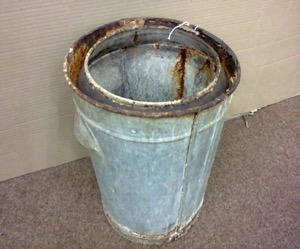
\includegraphics[width=\linewidth]{Mwaita_Figure_08}
	\caption{Cruelty treatment: Sanitary bucket.
  {\normalfont\scriptsize \\   Source: Robben Island Museum, Images taken by the author with permission of the museum.
                    }}
	\label{fig:Mwaita_Figure_08}
\end{figure}

Hand cuffs and leg irons are commonly used in imprisonment and or detention. Leg irons in and handcuffs in Figure \ref{fig:Mwaita_Figure_09} depict punishment and isolation. \textcite{Martin_2009} defined imprisonment and detention to “intentional practices that restrict individuals’ ability to move from one place to another and impose orders of space and time so that individual mobility is highly constrained, if not eliminated”. However, on Robben Island besides using hand cuffs to restrict prisoner’s movement, they were used for severely cruel punishment. Mr Salakatya Simuku \parencite[in][]{Robben_2003}, a former political prisoner from 1963 – 1966, described one of the uses of hand cuffs:

\blockcquote{Robben_2003}{Zolie Keke was amongst the youngest political prisoners during the early 1960's could not push the wheel barrow any more as his hands were full of blisters…He was taken to a shed nearby the quarry, three sets of hand cuffs were put on his hands and was asked to lie on a wooden plank that was designed like a triangle. He was beaten until he could not cry anymore from the beatings}

%Fig 9 AB
\begin{figure}[!htb]
	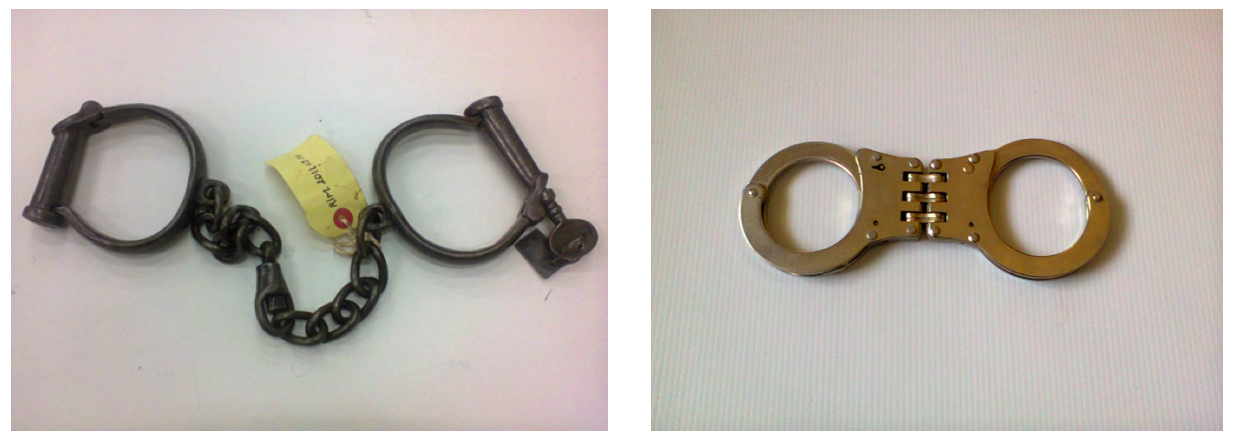
\includegraphics[width=\linewidth]{Mwaita_Figure_09}
	\caption{Punishment and isolation objects: leg irons (left) and hand cuffs (right).
  {\normalfont\scriptsize \\   Source: Robben Island Museum, Images taken by the author with permission of the museum.
                    }}
  	\label{fig:Mwaita_Figure_09}
\end{figure}

According to Simuka, when they heard that Zolile Keke was crying endlessly, the atmosphere in the quarry become tense, everybody looked at the shed and stopped working. A voice came loud saying ‘Ma Africa niyayibonana lento’ (Africans can you see what is happening?) \parencite{Robben_2003}. With such it can be seen that instead of the normal use of leg irons and hand cuffs to keep a prisoner from escaping they were also being used for merciless punishment on the Island.

\IJSRAsection{Challenges and Recommendations}

In providing a counter-narrative to the triumph interpretation the museum should display these objects of the brutality of apartheid political imprisonment on the Island. However, sea conditions and space shortage are logistical challenges to the broadening of the museum’s narrative. Although this is a challenge, there are ways of preserving vulnerable collections for the benefit of the present and future generations. One example has been outlined by a Conservator Toby Raphael during one of his training sessions at the International Centre for the Preservation and Restoration of Cultural Property (ICCROM) in 2005. He recommends that a properly engineered enclosure has an equally great potential for protecting and preserving vulnerable collections and is an efficient and often cost-effective way to meet conservation criteria for an object. When objects on display are housed in well designed and carefully fabricated cases, they can be effectively preserved at levels remarkably close to those provided in storage. The only difference from storage conditions is the exposure to light and this can be controlled as well \parencite[245--257]{Rafael_2005}.

\IJSRAsection{Conclusion}

Considering the above arguments that apartheid political imprisonment on Robben Island represents both the triumph of human spirit over adversity and a place of suffering and banishment, the current Robben Island Museum interpretation should be strengthened to include the tangible evidence that showcases the latter argument. It can be argued that the ‘triumphalism’ narrative is dominant at the expense of the inhumane and cruelty of apartheid political imprisonment era on the Island due to the absence of physical evidence in the form of material culture objects which can serve to remind and tell visitors of the cruelty of apartheid imprisonment. The current failure to attach memories to material culture objects can have negative effects for future interpretations because oral histories and memory tend to change with time and space leading to misinterpretation, while object tethered narratives are preserved through time in different ways. As such, it is very important for the Robben Island Museum to make use of its current repositories of rich memories and oral histories and to attach them to artefacts from its collections so that the objects may tell their stories.

\IJSRAclosing%<---- don’t change this!
